\documentclass[12pt]{article}
\usepackage{amsmath}
%\usepackage{fullpage}
\usepackage[top=1in, bottom=1in, left=0.8in, right=1in]{geometry}
\usepackage{multicol}
\usepackage{wrapfig}
\usepackage{graphicx}
\usepackage{float}
\usepackage{listings}
\usepackage{enumerate}
\lstset{language=Java,
basicstyle={\small\ttfamily},
columns=flexible,
belowskip=0mm}

\setlength{\columnsep}{0.1pc}

\title{ME573 Homework Set \# 6}
\author{Alexander Swenson -- \texttt{aaswenson@wisc.edu}}
\date{\today}
\begin{document}

  \maketitle

  \vspace{-0.3in}
  \noindent
  \rule{\linewidth}{0.4pt}

  \noindent
  
%%%%%%%%%%%%%%%%%%%%%%%%%%%%%%%%%%%%%%%%%%%%%%%%%%%%%%%%%%%%%%%%%%%%%%%%%%%%%%%%
% Problems 1

\section{Problem 1}

\noindent This problem solved the 1D heat diffusion equation using the Crank-Nicolson (CN) and the forward in time, central in space method (FTCS). Figure \ref{fig:problem1} shows the results of the schemes compared to the analytic solution. The $L_{\inf}$ error was calculated for both schemes. The CN error was 0.0676 and the FTCS error was 0.0513.

\begin{figure}[H]
	\centering
	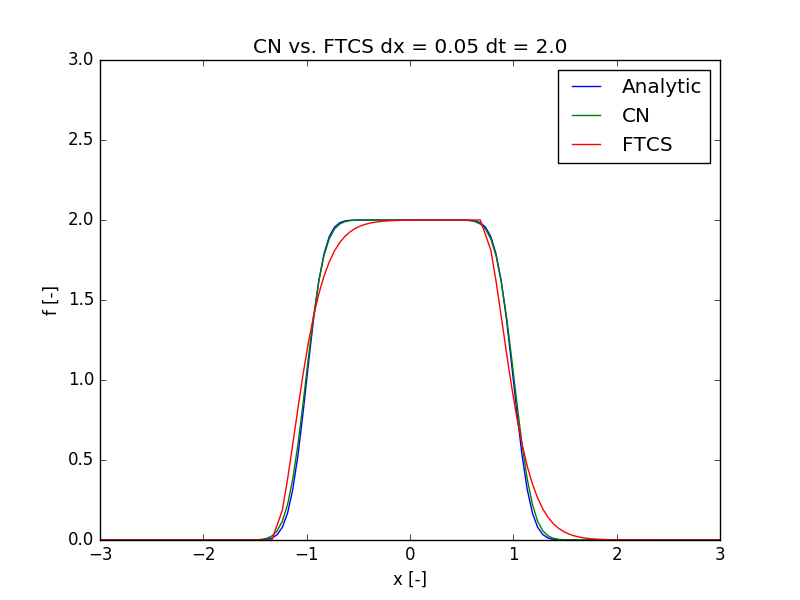
\includegraphics[height=3.75in]{problem1.png}
	\label{fig:problem1}
\end{figure}


%%%%%%%%%%%%%%%%%%%%%%%%%%%%%%%%%%%%%%%%%%%%%%%%%%%%%%%%%%%%%%%%%%%%%%%%%%%%%%%%


%%%%%%%%%%%%%%%%%%%%%%%%%%%%%%%%%%%%%%%%%%%%%%%%%%%%%%%%%%%%%%%%%%%%%%%%%%%%%%%%
% Problems:

\section{Problem 2}

\noindent This problem solved the 2D heat diffusion equation using the FTCS method. Figure \ref{fig:problem2a} shows the results of this scheme, after 80 time steps. Figure \ref{fig:problem2b} shows the $L_{\inf}$ error of the scheme. The maximum error was 0.05128. This error is too large and should be investigated.

\begin{figure}[H]
	\centering
	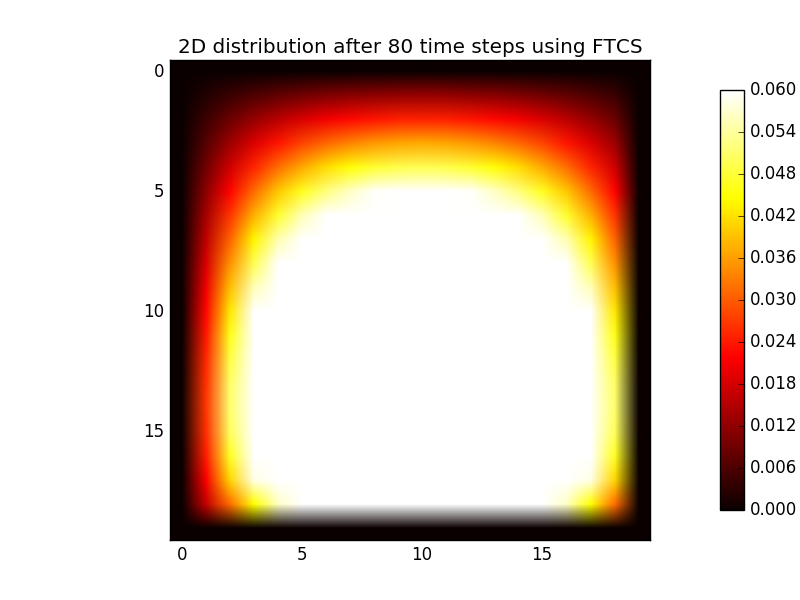
\includegraphics[height=3.75in]{problem2_plot.png}
	\label{fig:problem2_plot}
\end{figure}



\begin{figure}[H]
	\centering
	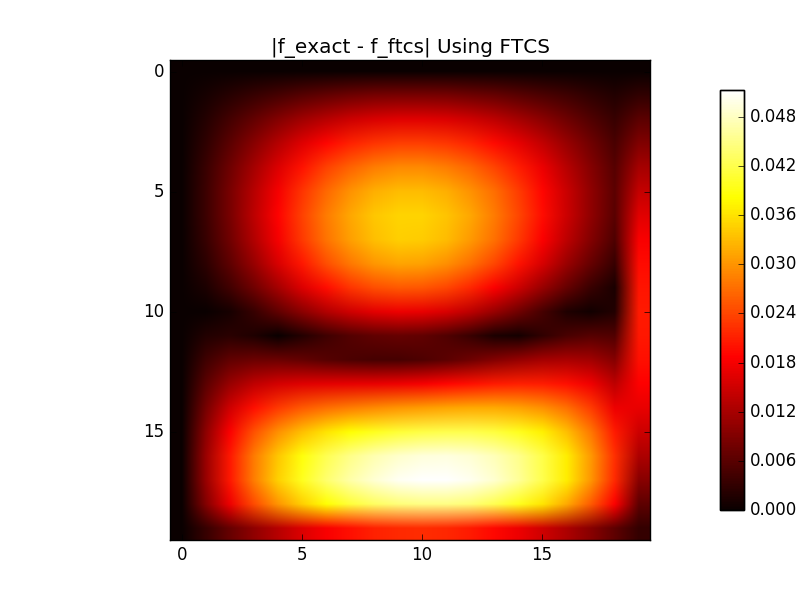
\includegraphics[height=3.75in]{problem2_error.png}
	\label{fig:problem2_error}
\end{figure}





\end{document}